\documentclass{article}
\usepackage{amsmath}
\usepackage{gensymb}
\usepackage{floatflt}
\setcounter{secnumdepth}{5}
\setlength{\textwidth}{5.0in}
\usepackage{setspace}
\usepackage{geometry}
\usepackage{graphicx}
\geometry{left=10mm,right=10mm}
\begin{document}
\title{Mathematical formulation of linear instability problem of a viscous incompressible  liquid round jet in a gaseous medium.}
\author{Srikumar Warrier}
%\affiliation{I.C.E.R, Indian Institute of Science, Bangalore}
%\begin{abstract}

%Linear Stability problem of a viscous incompressible round jet is setup.
%Governing equations are written in polar cylindrical coordinates and the linearised Navier stokes equations (LNS) are derived. %Boundary conditions and the interface matching conditions are presented.
%\end{abstract}
\maketitle
\section{Governing Equations.}
The continuity equation in polar cylindrical coordinates for the liquid phase is given by
\begin{equation}
\label{eq:conti1}
\frac{1}{r}\frac{\partial (ru_{r1})}{\partial r} + \frac{1}{r}\frac{\partial u_{\theta 1}}{\partial \theta} + \frac{\partial u_{z 1}}{\partial z} = 0
\end{equation}
For the gas phase,
\begin{equation}
\label{eq:conti2}
\frac{1}{r}\frac{\partial (ru_{r2})}{\partial r} + \frac{1}{r}\frac{\partial u_{\theta 2}}{\partial \theta} + \frac{\partial u_{z 2}}{\partial z} = 0
\end{equation}
The non dimensionalised momentum equation in the $r$ direction (radial direction) is given by 
\begin{equation}
\label{eq:rmom1}
\frac{\partial u_{r1}}{\partial t} + u_{r1}\frac{\partial u_{r1}}{\partial r} + \frac{u_{\theta 1}}{r}\frac{\partial u_{r1}}{\partial \theta} -\frac{u^2_{\theta 1}}{r} + u_{z 1}\frac{\partial u_{r 1}}{\partial z} = -\frac{\partial p}{\partial r}+ \frac{1}{Re_{1}}\Bigg[\frac{1}{r}\frac{\partial }{\partial r} \Bigg(r\frac{\partial u_{r1}}{\partial r}\Bigg)} - \frac{u_{r 1}}{r^2} + \frac{1}{r^2}\frac{\partial ^2 u_{r1}}{\partial \theta^2}}- \frac{2}{r^2}\frac{\partial u_{\theta 1}}{\partial \theta}+\frac{\partial^2 u_{r1}}{\partial z^2}\Bigg] 
\end{equation}
For the gas phase,
\begin{equation}
\label{eq:rmom2}
\frac{\partial u_{r2}}{\partial t} + u_{r2}\frac{\partial u_{r2}}{\partial r} + \frac{u_{\theta 2}}{r}\frac{\partial u_{r2}}{\partial \theta} -\frac{u^2_{\theta 2}}{r} + u_{z 2}\frac{\partial u_{r 2}}{\partial z} = -\frac{\partial p}{\partial r}+ \frac{1}{Re_{2}}\Bigg[\frac{1}{r}\frac{\partial }{\partial r}\Bigg (r\frac{\partial u_{r2}}{\partial r}\Bigg)} - \frac{u_{r 2}}{r^2} + \frac{1}{r^2}\frac{\partial ^2 u_{r2}}{\partial \theta^2}}- \frac{2}{r^2}\frac{\partial u_{\theta 2}}{\partial \theta}+\frac{\partial^2 u_{r2}}{\partial z^2}\Bigg] 
\end{equation}
In the azimuthal direction ($\theta$ direction),
\begin{equation}
\label{eq:azi1}
\frac{\partial u_{\theta1}}{\partial t} + u_{r1}\frac{\partial u_{\theta1}}{\partial r} + \frac{u_{\theta1}}{r}\frac{\partial u_{\theta1}}{\partial \theta} +\frac{u_{\theta1}u_{r1}}{r} + u_{z1}\frac{\partial u_{\theta1}}{\partial z} = -\frac{1}{r}\frac{\partial p}{\partial \theta}+ \frac{1}{Re_{1}}\Bigg[\frac{1}{r}\frac{\partial }{\partial r} \Bigg( r\frac{\partial u_{\theta1}}{\partial r}\Bigg) - \frac{u_{\theta1}}{r^2} + \frac{1}{r^2}\frac{\partial ^2 u_{\theta1}}{\partial \theta^2}}+ \frac{2}{r^2}\frac{\partial u_{r1}}{\partial \theta}+\frac{\partial^2 u_{\theta1}}{\partial z^2}\Bigg]
\end{equation}
For the gas phase,
\begin{equation}
\label{eq:azi2}
\frac{\partial u_{\theta2}}{\partial t} + u_{r2}\frac{\partial u_{\theta2}}{\partial r} + \frac{u_{\theta2}}{r}\frac{\partial u_{\theta2}}{\partial \theta} +\frac{u_{\theta2}u_{r2}}{r} + u_{z2}\frac{\partial u_{\theta2}}{\partial z} = -\frac{1}{r}\frac{\partial p}{\partial \theta}+ \frac{1}{Re_{2}}\Bigg[\frac{1}{r}\frac{\partial }{\partial r} \Bigg( r\frac{\partial u_{\theta2}}{\partial r}\Bigg) - \frac{u_{\theta2}}{r^2} + \frac{1}{r^2}\frac{\partial ^2 u_{\theta2}}{\partial \theta^2}}+ \frac{2}{r^2}\frac{\partial u_{r2}}{\partial \theta}+\frac{\partial^2 u_{\theta2}}{\partial z^2}\Bigg]
\end{equation}
In the axial direction ($z$ direction) for the liquid phase
\begin{equation}
\label{eq:axi1}
\frac{\partial u_{z1}}{\partial t} + u_{r1}\frac{\partial u_{z1}}{\partial r} + \frac{u_{\theta1}}{r}\frac{\partial u_{z1}}{\partial \theta}  + u_{z1}\frac{\partial u_{z1}}{\partial z} = -\frac{\partial p}{\partial z}+ \frac{1}{Re_{1}}\Bigg[\frac{1}{r}\frac{\partial }{\partial r} \Bigg(r\frac{\partial u_{z1}}{\partial r}\Bigg)} + \frac{1}{r^2}\frac{\partial ^2 u_{z1}}{\partial \theta^2}}+\frac{\partial^2 u_{z1}}{\partial z^2}\Bigg]
\end{equation}
For the gas phase,
\begin{equation}
\label{eq:axi2}
\frac{\partial u_{z2}}{\partial t} + u_{r2}\frac{\partial u_{z2}}{\partial r} + \frac{u_{\theta2}}{r}\frac{\partial u_{z2}}{\partial \theta}  + u_{z2}\frac{\partial u_{z2}}{\partial z} = -\frac{\partial p}{\partial z}+ \frac{1}{Re_{2}}\Bigg[\frac{1}{r}\frac{\partial }{\partial r} \Bigg(r\frac{\partial u_{z2}}{\partial r}\Bigg)} + \frac{1}{r^2}\frac{\partial ^2 u_{z2}}{\partial \theta^2}}+\frac{\partial^2 u_{z2}}{\partial z^2}\Bigg]
\end{equation}
where $u_{r}$ , $u_{\theta}$ and $u_{z}$ are the velocity components in the radial, azimuthal and axial directions respectively.
\section{Base flow.}
The flow variables are assumed to consist of a mean part and an infinitesimally small perturbation.
\begin{equation}
\begin{align}
\begin{split}
  u_{r} = U_{r} + u'_{r}(r,\theta,z,t) \\
  u_{\theta} = U_{\theta} +u'_{\theta}(r,\theta,z,t) \\
  u_{z} = U_{z}+ u'_{z}(r,\theta,z,t)  
\end{split}
\end{align}
\end{equation}

The base flow is taken to be an incompressible viscous axisymmetric one with locally parallel flow assumption.
The base flow quantities are
\begin{equation}
\begin{split}
U_{r1} = U_{r1}(r) \\
U_{r2} = U_{r2}(r) \\
U_{\theta} = 0 \\
U_{z1} = U_{z1}(r) \\ 
U_{z2} = U_{z2}(r) \\
P = 0 \\
\end{split}
\end{equation}
\subsection{Normal mode form of perturbation.}
The flow is periodic in azimuthal and axial direction. We assume perturbations of the form 
\begin{equation}
\label{eq:normalmode}
[u_{r},u_{\theta},u_{z},p] = [i\tilde {u}_{r} (r), \tilde {u}_{\theta} (r), \tilde {u}_{z} (r),\tilde{p}(r)]e^{i(\alpha z + m\theta - \omega t)}
\end{equation}
It is to be noted that $u_{r}\propto i\tilde{u}_{r} $ . This can be readily seen from the contunity equation, the phase of $u_{r} $ differs by $\frac{\pi}{2}$ from that of $ u_{\theta}$ and $u_{r}.$
Substituting eq(\ref{eq:normalmode}) into eq(\ref{eq:rmom1}), eq(\ref{eq:rmom2}), eq(\ref{eq:azi1}), eq(\ref{eq:azi2}), eq(\ref{eq:axi1}), eq(\ref{eq:axi2}) , eq(\ref{eq:conti1}) and eq(\ref{eq:conti2}), we have,
In the radial direction,
\begin{equation}
\label{rlinear1}
-i\frac{\tilde{u}_{r1}''}{Re_{1}} + i\Bigg( U_{r1}-\frac{1}{rRe_{1}}\Bigg)\tilde{u}_{r1}' +
\Bigg[\omega + iU_{r1}' - \alpha U_{z1} + \frac{i}{Re_{1}}\Bigg(\frac{m^2 + 1}{r^2}+ \alpha ^2\Bigg)\Bigg]\tilde{u}_{r1} +  {\frac{2im}{r^2Re_{1}}}\tilde{u}_{\theta1} + \tilde{p}' = 0
\end{equation}
\begin{equation}
\label{rlinear2}
-i\frac{\tilde{u}_{r2}''}{Re_{2}} + i\Bigg( U_{r2}-\frac{1}{rRe_{2}}\Bigg)\tilde{u}_{r2}' +
\Bigg[\omega + iU_{r2}' - \alpha U_{z2} + \frac{i}{Re_{2}}\Bigg(\frac{m^2 + 1}{r^2}+ \alpha ^2\Bigg)\Bigg]\tilde{u}_{r2} +  {\frac{2im}{r^2Re_{2}}}\tilde{u}_{\theta2} + \tilde{p}' = 0
\end{equation}
In the azimuthal direction,
\begin{equation}
\label{azilinear1}
-\frac{\tilde{u}_{\theta 1}''}{Re_{1}} + \Bigg( U_{r1}-\frac{1}{rRe_{1}}\Bigg)\tilde{u}_{\theta 1}' +
\Bigg[-i\omega + i\alpha U_{z1} +\frac{U_{r1}}{r} + \frac{1}{Re_{1}}\Bigg(\frac{m^2 + 1}{r^2}+ \alpha ^2\Bigg)\Bigg]\tilde{u}_{\theta 1} +  \Bigg(\frac{2m}{r^2Re_{1}}}\Bigg)\tilde{u}_{r1} + \frac{im\tilde{p}}{r} = 0
\end{equation}
\begin{equation}
\label{azilinear2}
-\frac{\tilde{u}_{\theta2}''}{Re_{2}} + \Bigg( U_{r2}-\frac{1}{rRe_{2}}\Bigg)\tilde{u}_{\theta 2}' +
\Bigg[-i\omega + i\alpha U_{z2} +\frac{U_{r2}}{r} + \frac{1}{Re_{2}}\Bigg(\frac{m^2 + 1}{r^2}+ \alpha ^2\Bigg)\Bigg]\tilde{u}_{\theta 2} +  \Bigg(\frac{2m}{r^2Re_{2}}}\Bigg)\tilde{u}_{r2} + \frac{im\tilde{p}}{r} = 0
\end{equation}
In the axial direction,
\begin{equation}
\label{axilinear1}
-\frac{\tilde{u}_{z1}''}{Re_{1}} + \Bigg( U_{r1}-\frac{1}{rRe_{1}}\Bigg)\tilde{u}_{z1}' +
\Bigg[-i\omega + i\alpha U_{z1}  + \frac{1}{Re_{1}}\Bigg(\frac{m^2}{r^2}+ \alpha ^2\Bigg)\Bigg]\tilde{u}_{z1} + iU_{z1}'\tilde{u}_{r1} + i\alpha \tilde{p} = 0
\end{equation}
\begin{equation}
\label{axilinear2}
-\frac{\tilde{u}_{z2}''}{Re_{2}} + \Bigg( U_{r2}-\frac{1}{rRe_{2}}\Bigg)\tilde{u}_{z2}' +
\Bigg[-i\omega + i\alpha U_{z2}  + \frac{1}{Re_{2}}\Bigg(\frac{m^2}{r^2}+ \alpha ^2\Bigg)\Bigg]\tilde{u}_{z2} + iU_{z2}'\tilde{u}_{r2} + i\alpha \tilde{p} = 0
\end{equation}
Continuity equation yields,
\begin{equation}
\label{linearconti}
\tilde{u}_{r1}' + \frac{\tilde{u}_{r1}}{r} + \frac{m\tilde{u}_{\theta 1}}{r}+ 
\alpha \tilde{u}_{z1} = 0
\end{equation}
\begin{equation}
\label{linearconti}
\tilde{u}_{r2}' + \frac{\tilde{u}_{r2}}{r} + \frac{m\tilde{u}_{\theta 2}}{r}+ 
\alpha \tilde{u}_{z2} = 0
\end{equation}

\section{Boundary Conditions.}
Due to the singular nature of the coordinate system on the centerline, all physical quantities must be smooth and bounded at $r$ = 0 .Therefore as   $r$ \rightarrow{0},
\begin{equation}
\lim _{r\rightarrow {0}}\frac{\partial \bf V}{\partial \theta} = 0.
\end{equation}
\begin{equation}
\lim_{r\rightarrow{0}}\frac{\partial p'}{\partial \theta} = 0
\end{equation}

where  {\bf V} is the total velocity vector. the above limits represents the boundedness and smoothness conditions on the solutions along the centerline.(Batchelor and Gill 1962, also Khorrami et al.,JCP 81,206-229 (1989)).  
while expanding the limits, we need to consider only the perturbation part of the velocity since the mean flow is independent of $z$ and $\theta$
\begin{equation*}
\lim _{r\rightarrow {0}}\frac{\partial \bf V}{\partial \theta} = \lim_{r\rightarrow{0}}\frac{\partial}{\partial \theta}(u_{r1}{\bf e_{r}} + u_{\theta 1}{\bf e_{\theta}} + u_{z1}{\bf e_{z}}) = 0
\end{equation*}
But 
\begin{equation}
\frac{\partial {\bf e_{z}}}{\partial \theta} = 0; \frac{\partial {\bf e_{r}}}{\partial \theta} ={\bf e_{\theta}}; \frac{\partial {\bf e_{\theta}}}{\partial \theta} = -{\bf e_{r}}
\end{equation}
\begin{equation*}
-(m\tilde{u}_{r1}){\bf e_{r}} + i(\tilde{u}_{r1}+m\tilde{u}_{\theta1}){\bf e_{\theta}} + in\tilde{u}_{z1}{\bf e_{z}}=0
\end{equation*}
\begin{equation*}
imp = 0
\end{equation*}
In order for the inequality to hold, each component of the resultant vector must be zero. This gives,
\begin{equation}
m\tilde{u}_{r1}=0
\end{equation}
\begin{equation}
\tilde{u}_{r1}+m\tilde{u}_{\theta1} = 0
\end{equation}
\begin{equation}
m\tilde{u}_{z1} =0
\end{equation}
\begin{equation}
mp = 0
\end{equation}
For axisymmetric perturbation $m = 0$,
\begin{equation}
\tilde{u}_{r1}(0) = \tilde{u}_{\theta1}(0) = 0 
\end{equation}
$ \tilde{u}_{z1}(0)$ and $\tilde{p}(0)$ must be finite.
and for $m =\pm 1$
\begin{equation}
\tilde{u}_{r1}(0) \pm  \tilde{u}_{\theta1}(0) = 0 
\end{equation}
\begin{equation}
 \tilde{u}_{z1}(0)=\tilde{p}(0)=0
\end{equation}
if $|m| > 1$,
\begin{equation}
 \tilde{u}_{z1}(0)=\tilde{p}(0)=0
\end{equation}
\begin{equation}
\tilde{u}_{r1}(0)= \tilde{u}_{\theta1}(0) = 0
\end{equation}
In case when $|m| =1$, continuity equation is applied on the centerline with $\tilde{u}_{z} = 0$ which gives,
\begin{equation}
2\tilde{u}_{r1}'(0) + m\tilde{u}_{\theta1}'(0) = 0
\end{equation}

\subsection{Matching Conditions at the interface.}
Let
\begin{equation}
\phi(r,z,\theta,t) = h(z,\theta,t) - r
\end{equation}
so that the 0 level set of $\phi $ describes the interface between the liquid jet and the gaseous medium. The  Kinematic  condition that the interface is a material surface gives ,
\begin{equation}
\frac{D\phi}{Dt} = 0
\end{equation}
\begin{equation}
\label{interfaceevol}
\frac{\partial{h}}{\partial{t}} + \frac{u_{\theta}}{r}\frac{\partial{h}}{\partial{\theta}} + u_{z}\frac{\partial{h}}{\partial{z}} = \Bigg(\frac{\partial{r}}{\partial{t}}\Bigg)_{r=R} = u_{r}(h(z,\theta,t),\theta ,z,t)
\end{equation}

We assume wave-like perturbation of the interface as 

\begin{equation}
\label{interface}
h'(z,\theta,t) = \tilde{h}e^{i(\alpha z + m\theta - \omega t)}
 \end{equation}


\begin{equation}
h = \overline h(z) + h'(z,\theta,t)
\end{equation}

Substituting eq(\ref{interface}) in eq(\ref{interfaceevol}) and subtracting the mean flow  we get,

\begin{equation}
\begin{split}
\frac{\partial h'(z,\theta ,t)}{\partial t} + \frac{u'_{\theta}(h(z,\theta, t),z,\theta,t)}{r}\bigg(\frac{\partial h'(z ,\theta,t)}{\partial \theta}\bigg)  +  U_{z}(r)\bigg(\frac{\partial h'(z,\theta ,t)}{\partial z}\bigg) + u'_{z}(h(z,\theta,t),\theta,z,t)\frac{d\overline{h}(z)}{dz} + \\
 u'_{z}(h(z,\theta,t),\theta,z,t)\frac{\partial h'(z,\theta,t)}{\partial z} =  u'_{r}(h(z,\theta,t),\theta ,z,t)
\end{split}
\end{equation}


The above equation is nonlinear in $h$ as $ u'_{z}$ and $ u'_{\theta}$ are functions of $ h,\theta,z,t$.
%expanding we get,

%\begin{equation}
%\frac{\partial{h'(z,\theta,t)}}{\partial{t}} + \frac{u'_{\theta}}{r}\frac{\partial{h'(z,\theta,t)}}{\partial{\theta}} + U_{z} %(r)\frac{\partial{h'(z,\theta,t)}}{\partial{z}} + u'_{z}\frac{\partial{h'(z,\theta,t)}}{\partial{z}} = u_{r}(h(z,\theta,t), %\theta %,z,t) 
%\end{equation}


For infintesimally small perturbation , we linearise the above equation as , 

\begin{equation}
\frac{\partial{h'(z,\theta,t)}}{\partial{t}} + U_{z}(r)\frac{\partial{h'(z,\theta,t)}}{\partial{z}} + u'_{z}(h(z,\theta , t),z,\theta ,t)\frac{d\overline{h}(z)}{dz} = u'_{r}(h(z,\theta,t),\theta ,z,t)
\end{equation}


Substituting normal mode form of perturbation, we get,

\begin{equation}
-i\omega \tilde{h} e^{i(\alpha z + m\theta - \omega t)} + i\alpha  U_{z}(r)\tilde{h} e^{i(\alpha z + m\theta - \omega t)} + \tilde{u}_{z} e^{i(\alpha z + m\theta - \omega t)}\frac{d\overline{h}(z)}{dz} = \tilde{u}_{r}(h(z,\theta,t))e^{i(\alpha z + m\theta - \omega t)}
\end{equation}
or ,

\begin{equation}
-i\omega \tilde{h}  + i\alpha  U_{z}(r)\tilde{h}  + \tilde{u}_{z}\frac{d\overline{h}(z)}{dz}  = \tilde{u}_{r}(h(z,\theta,t))
\end{equation}

At the interface, we can write ,
\begin{equation}
-i\omega \tilde{h} + i\alpha \tilde{h}U_{z1}(r) + \tilde{u}_{z1}\frac{d\overline{h}(z)}{dz} = \tilde{u}_{r1}(h(z,\theta , t))
\end{equation}
\begin{equation}
-i\omega \tilde{h} + i\alpha \tilde{h}U_{z2}(r) + \tilde{u}_{z2}\frac{d\overline{h}(z)}{dz} = \tilde{u}_{r2}(h(z,\theta , t))
\end{equation}
\section{Stress boundary conditions}
The normal stress in terms of the local pressure and velocity field is given by 
\begin{equation}
\label{tau}
\tau = -pI + \mu[(\nabla u)+ (\nabla u)^T]
\end{equation}
where,
\begin{equation}
\nabla u = \bigg({\bf e_{r}\frac{\partial}{\partial r} + \frac{{\bf e_{\theta}}}{r}\frac{\partial }{\partial \theta } + {\bf e_{z}}}\frac{\partial}{\partial z}\bigg)(u_{r}{\bf e_{r}} + u_{\theta}{\bf e_{\theta}} + u_{z}{\bf e_{z}}) 
\end{equation}
\begin{equation}
\label{gradu}
\nabla u = {\bf e_{r}}\frac{\partial}{\partial r} (u_{r}{\bf e_{r}} + u_{\theta}{\bf e_{\theta}} + u_{z}{\bf e_{z}}) + \frac{{\bf e_{\theta}}}{r}\frac{\partial}{\partial \theta} (u_{r}{\bf e_{r}} + u_{\theta}{\bf e_{\theta}} + u_{z}{\bf e_{z}}) 
+ {\bf e_{z}}\frac{\partial}{\partial z} (u_{r}{\bf e_{r}} + u_{\theta}{\bf e_{\theta}} + u_{z}{\bf e_{z}})
\end{equation}
The following identities are to be noted, 

\begin{equation*}
\frac{\partial {\bf e_{r}}}{\partial r} = 0;  \frac{\partial {\bf e_{\theta}}}{\partial r} = 0; \frac{\partial {\bf e_{z}}}{\partial r} =0;
\end{equation*}
\begin{equation*}
\frac{\partial {\bf e_{r}}}{\partial \theta} ={\bf e_{\theta}}; \frac{\partial {\bf e_{\theta}}}{\partial \theta} = -{\bf e_{r}};    
\frac{\partial {\bf e_{z}}}{\partial \theta} = 0;
\end{equation*}
\begin{equation*}
\frac{\partial {\bf e_{r}}}{\partial z} = 0;  \frac{\partial {\bf e_{\theta}}}{\partial z} = 0; \frac{\partial {\bf e_{z}}}{\partial z} =0;
\end{equation*}  
We evaluate eq(\ref{gradu}) term by term by using the above identities
\begin{equation}
{\bf e_{r}}\frac{\partial}{\partial r} (u_{r}{\bf e_{r}} + u_{\theta}{\bf e_{\theta}} + u_{z}{\bf e_{z}}) = {\bf e_{r}}{\bf e_{r}}
\frac{\partial u_{r}}{\partial r} + {\bf e_{r}}{\bf e_{\theta}}\frac{\partial u_{\theta}}{\partial r} + {\bf e_{r}}{\bf e_{z}}
\frac{\partial u_{z}}{\partial r}
\end{equation}

\begin{equation}
\frac{{\bf e_{\theta}}}{r} \frac{\partial}{\partial \theta} (u_{r}{\bf e_{r}} + u_{\theta}{\bf e_{\theta}} + u_{z}{\bf e_{z}}) = {\bf e_{\theta} e_{r}}\bigg(\frac{1}{r}\frac{\partial u_{r}}{\partial \theta}\bigg) + {\bf e_{\theta}{e_{\theta}}}\bigg(\frac{u_{r}}{r}\bigg) + {\bf e_{\theta}{e_{\theta}}}\bigg(\frac{1}{r}\frac{\partial u_{\theta}}{\partial \theta}\bigg) - {\bf e_{\theta} e_{r}}}\bigg(\frac{u_{\theta}}{r}\bigg) + {\bf e_{\theta}{e_{z}}}\bigg(\frac{1}{r}\frac{\partial u_{z}}{\partial \theta}\bigg) 
\end{equation}

\begin{equation}
{\bf e_{z}}\frac{\partial}{\partial z} (u_{r}{\bf e_{r}} + u_{\theta}{\bf e_{\theta}} + u_{z}{\bf e_{z}}) = {\bf e_{z}}{\bf e_{r}}
\frac{\partial u_{r}}{\partial z} + {\bf e_{z}}{\bf e_{\theta}}\frac{\partial u_{\theta}}{\partial z} + {\bf e_{z}}{\bf e_{z}}
\frac{\partial u_{z}}{\partial z}
\end{equation}

\begin{equation}
\label{nablau}
\nabla u =
\begin{bmatrix} 
\frac{\partial u_{r}}{\partial r}   &  \frac{\partial u_{\theta}}{\partial r} & \frac{\partial u_{z}}{\partial r} \\
\bigg(\frac{1}{r}\frac{\partial u_{r}}{\partial \theta} -\frac{u_{\theta}}{r}\bigg) & \bigg(\frac{u_{r}}{r}+\frac{1}{r}\frac{\partial u_{\theta}}{\partial \theta}\bigg)  & \frac{1}{r}\frac{\partial u_{z}}{\partial \theta} \\
\frac{\partial u_{r}}{\partial z} &  \frac{\partial u_{\theta}}{\partial z} & \frac{\partial u_{z}}{\partial z}
\end{bmatrix}
\end{equation}

\begin{equation}
\label{nablautrans}
(\nabla u)^T =
\begin{bmatrix} 
\frac{\partial u_{r}}{\partial r}   & \bigg(\frac{1}{r}\frac{\partial u_{r}}{\partial \theta} -\frac{u_{\theta}}{r}\bigg) &   \frac{\partial u_{r}}{\partial z}\\
\frac{\partial u_{\theta}}{\partial r} & \bigg(\frac{u_{r}}{r}+\frac{1}{r}\frac{\partial u_{\theta}}{\partial \theta}\bigg)  &       \frac{\partial u_{\theta}}{\partial z}  \\
\frac{\partial u_{z}}{\partial r} & \frac{1}{r}\frac{\partial u_{z}}{\partial \theta}  & \frac{\partial u_{z}}{\partial z}
\end{bmatrix}
\end{equation}

\begin{equation}
[\nabla u + (\nabla u)^T] =
\begin{bmatrix}
2\frac{\partial u_{r}}{\partial r}   &  \bigg(\frac{1}{r}\frac{\partial u_{r}}{\partial \theta} -\frac{u_{\theta}}{r}+\frac{\partial u_{\theta}}{\partial r}\bigg) & \bigg(\frac{\partial u_{z}}{\partial r} + \frac{\partial u_{r}}{\partial z}\bigg) \\
\bigg(\frac{1}{r}\frac{\partial u_{r}}{\partial \theta} -\frac{u_{\theta}}{r}+\frac{\partial u_{\theta}}{\partial r}\bigg) & 2\bigg(\frac{u_{r}}{r}+\frac{1}{r}\frac{\partial u_{\theta}}{\partial \theta}\bigg)  & \bigg(\frac{1}{r}\frac{\partial u_{z}}{\partial \theta} + \frac{\partial u_{\theta}}{\partial z}\bigg) \\
\bigg(\frac{\partial u_{z}}{\partial r} + \frac{\partial u_{r}}{\partial z}\bigg) &  \bigg(\frac{1}{r}\frac{\partial u_{z}}{\partial \theta} + \frac{\partial u_{\theta}}{\partial z}\bigg) & 2\frac{\partial u_{z}}{\partial z}
\end{bmatrix} 
\end{equation}

\therefore eq(\ref{tau}) becomes ,
\begin{equation}
\tau =
\begin{bmatrix}
-p + 2\mu \frac{\partial u_{r}}{\partial r}   &  \mu \bigg(\frac{1}{r}\frac{\partial u_{r}}{\partial \theta} -\frac{u_{\theta}}{r}+\frac{\partial u_{\theta}}{\partial r}\bigg) & \mu \bigg(\frac{\partial u_{z}}{\partial r} + \frac{\partial u_{r}}{\partial z}\bigg) \\
\mu \bigg(\frac{1}{r}\frac{\partial u_{r}}{\partial \theta} -\frac{u_{\theta}}{r}+\frac{\partial u_{\theta}}{\partial r}\bigg) & -p + 2\mu \bigg(\frac{u_{r}}{r}+\frac{1}{r}\frac{\partial u_{\theta}}{\partial \theta}\bigg)  & \mu \bigg(\frac{1}{r}\frac{\partial u_{z}}{\partial \theta} + \frac{\partial u_{\theta}}{\partial z}\bigg) \\
\mu \bigg(\frac{\partial u_{z}}{\partial r} + \frac{\partial u_{r}}{\partial z}\bigg) &  \mu \bigg(\frac{1}{r}\frac{\partial u_{z}}{\partial \theta} + \frac{\partial u_{\theta}}{\partial z}\bigg) & -p + 2\mu \frac{\partial u_{z}}{\partial z}
\end{bmatrix} 
\end{equation}

\subsection{Stress balance conditions at the liquid-gas interface.}
We now derive the normal and tangential stress conditions at the liquid-gas interface.
Consider an interfacial surface S bounded by a closed curve C.  Surface tension $\sigma$ is defined as the force per unit length in the s-direction at every point along C that acts to flatten the surface S.  Performing a force balance on a volume element V enclosing the interfacial surface S  defined by the contour C : \newline
\begin{figure}[b] 
  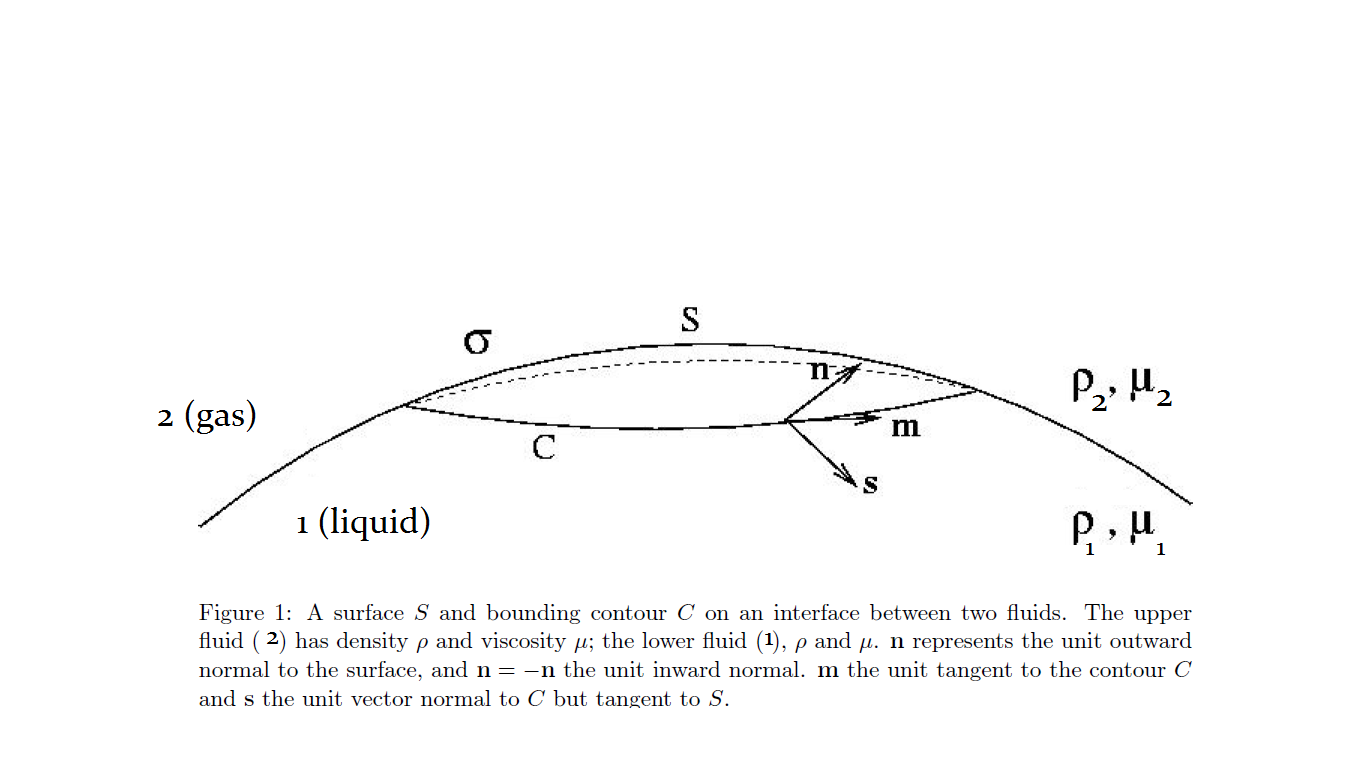
\includegraphics[scale=0.5]{interface1.png}
\end{figure}
\newline
\begin{equation}
\int_V \rho\frac{D{\bf u}}{Dt} dV = \int_V f dV + \int_S [{\bf(t_{1}(n))} + {\bf(t_{2}(n))}] dS + \int_C \sigma {\bf s} dl
\end{equation}
$dl$ is elemental length segment along the curve C. 
${\bf \tau} = -pI + \mu[(\nabla u)+ (\nabla u)^T]$ is the total normal stress tensor.
${\bf t_{1}(n)} ={\bf -n\cdot\tau_{1}}$ is the total normal stress vector exerted by the liquid phase on the interface  while ${\bf t_{2}(n)} ={\bf n\cdot\tau_{2}}$ is the total normal stress vector exerted by the gas phase on the interface.
Now if $\epsilon $ is the typical length scale of the element V ,then the acceleration and body forces will scale as $\epsilon^3$, while the surface forces scale as $\epsilon^2$. Hence in the limit of $\epsilon \rightarrow 0$, only the surface forces must balance,
\begin{figure}[H]
  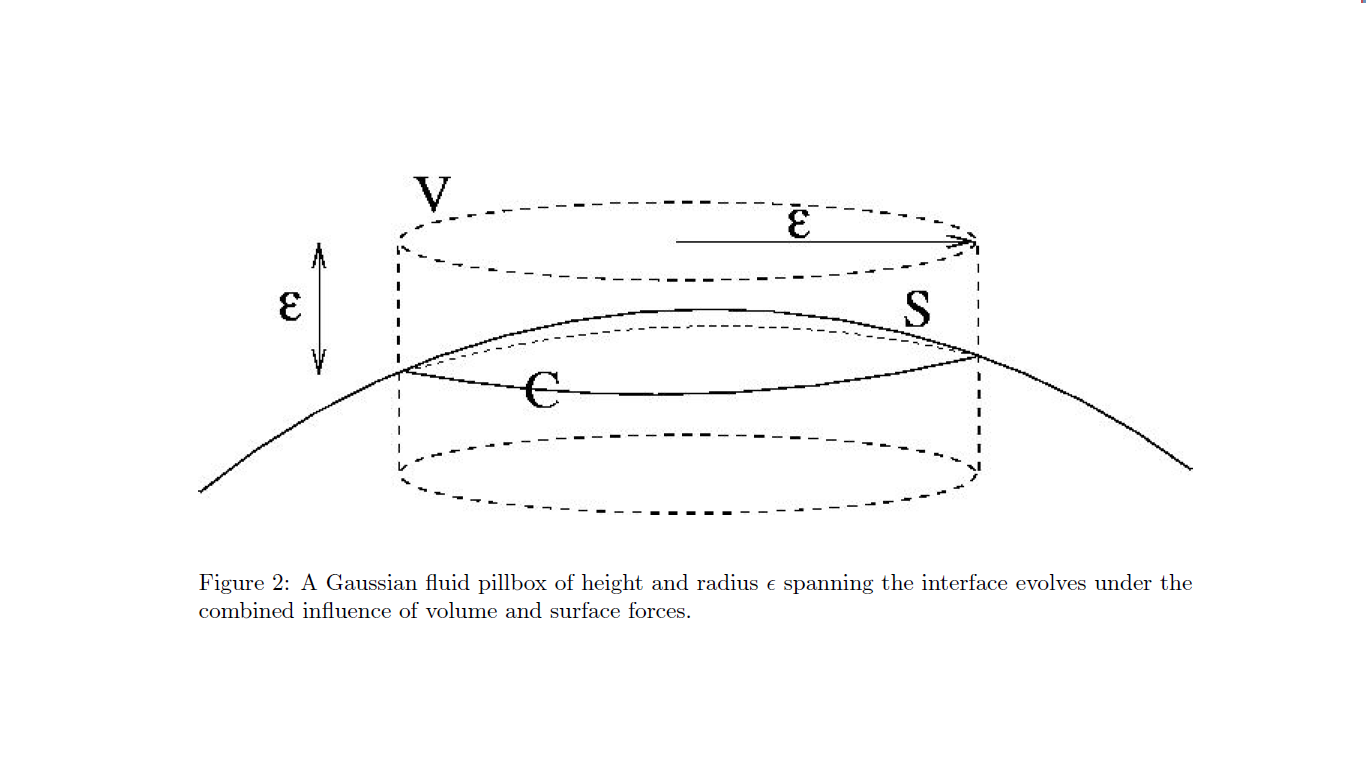
\includegraphics[width=6.5in]{pillbox.png}
\end{figure}
\begin{equation}
\label{force balance}
\int_S [{\bf(t_{1}(n))} + {\bf(t_{2}(n))}] dS + \int_C \sigma {\bf s} dl = 0 
\end{equation}
consider $\int_C \sigma {\bf s} dl $ . using stokes theorem we can write ,
\begin{equation}
\int_C \sigma {\bf s} dl = \int_S {\bf n\sigma(\nabla \cdot {\bf n}})ds 
\end{equation}
\subsection*{\bf proof}
From stokes theorem we know that,
\begin{equation*}
\int_C {\bf F \cdot dl} = \int_S {\bf n \cdot (\nabla \times F)}ds
\end{equation*} 
Along the curve C, $ {\bf dl} = {\bf m}dl$
\begin{equation*}
\int_C {\bf F \cdot m}dl = \int_s {\bf n \cdot (\nabla \times F)}ds
\end{equation*}
choose ${\bf F = f \times b}$. Where ${\bf b}$ is an arbitrary constant vector.
\begin{equation*}
\int_C {\bf (f \times b).m}dl = \int_S {\bf n \cdot (\nabla \times (f \times b))} ds
\end{equation*}

using the vector identities ,
\begin{equation}
{\bf A\cdot(B \times C) = -B\cdot(A \times C)}
\end{equation}

\begin{equation}   
{\bf \nabla \times (A\times B) = A(\nabla \cdot B)-B(\nabla \cdot A) + (B \cdot \nabla)A - (A \cdot \nabla)B}
\end{equation}
\newline

the LHS can be written $\int_C {\bf (f \times b).m}dl = \int_C {\bf -b \cdot (f \times m)}dl$, 
the RHS can be written as \newline

$\int_S {\bf n \cdot [f(\nabla \cdot b) - b(\nabla \cdot f) + (b \cdot \nabla f) -(f \cdot \nabla b)}ds$
\newline
 
since ${\bf b}$ is an constant vector  $(\nabla \cdot b) = 0$ and $\nabla b = 0$ 

\begin{equation}
\int_C {\bf -b \cdot (f \times m)}dl = \int_S {\bf n \cdot (-b(\nabla \cdot f) + (b \cdot \nabla f))}ds
\end{equation}

since ${\bf b}$ is an arbitrary vector 
\begin{equation}
b \cdot \int_C {\bf  (f \times m)}dl = b \cdot \int_S {\bf (n(\nabla \cdot f) - ( n \cdot \nabla f))}ds
\end{equation}

choose ${\bf f} =\sigma{\bf n}$.
\begin{equation}
\int_C (\sigma{\bf n \times m})dl = \int_S[{\bf n(\nabla \cdot}\sigma{\bf n) - (n \cdot \nabla}\sigma{\bf n})] ds
\end{equation} 

we note the following, 
\begin{itemize}
\item[1)]$ {\bf \nabla \cdot}\sigma {\bf n} = \nabla \sigma \cdot {\bf n} + \sigma {\bf \nabla \cdot n}$. 
\item[2)]$ {\bf \nabla }(\sigma {\bf n}) = \sigma {\bf \nabla n  +  n\nabla }\sigma$.
\item[3)]$ {\bf n \times m = -s}$ 
\item[4)]$ \nabla \sigma \cdot {\bf n} = 0 $
\item[5)]$ {\bf \nabla n \cdot n = \frac{1}{2}\nabla (n \cdot n)} = 0 $
\item[6)] We assume that $\nabla \sigma = 0 $
\end{itemize}

This yields, \newline

\begin{equation*}
-\int_C \sigma {\bf s}dl = \int_S{\bf n }\sigma {\bf (\nabla \cdot n)} ds
\end{equation*}

 \textit{end of proof. }
 \begin{figure}[H] 
  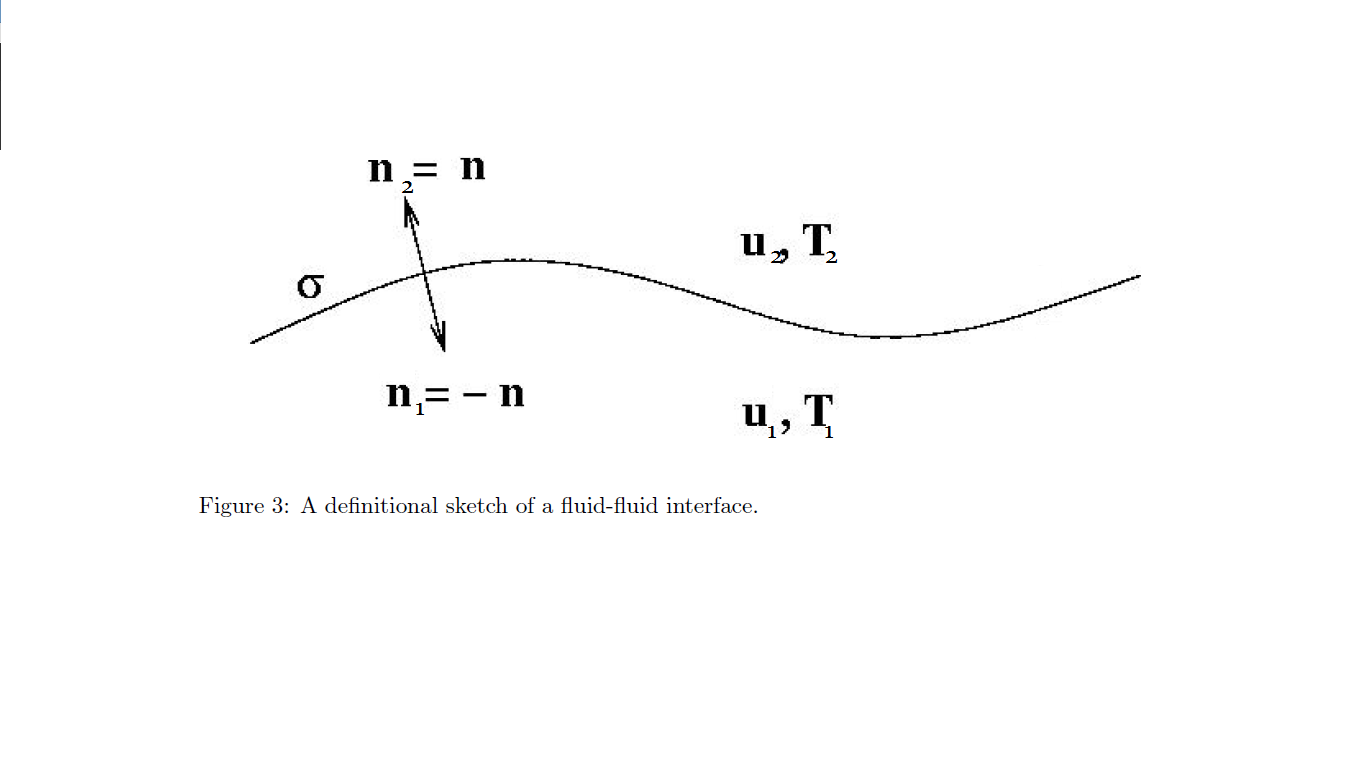
\includegraphics[width=6.5in]{interface2.png}
\end{figure}
\newpage

Rewriting eq(\ref {force balance}), 
\begin{equation*}
\int_S [{\bf(t_{1}(n))} + {\bf(t_{2}(n))}] dS + \int_C \sigma {\bf s} dl = 0
\end{equation*}

\begin{equation}
\int_ S [{\bf n \cdot \tau_{2}} - {\bf n\cdot \tau_{1}}]ds - \int_S{\bf n }\sigma {\bf (\nabla \cdot n)} ds = 0
\end{equation}
Since the surface element is arbitrary , the integral must vanish identically.
\begin{equation}
\label{stress balance}
{\bf {\bf n \cdot \tau_{2}} - {\bf n\cdot \tau_{1}} = {\bf n}\sigma {\bf (\nabla \cdot n)}}
\end{equation}
\subsection{Normal stress balance}
Taking ${\bf n \cdot}(eq {\ref {stress balance}})$  yields the normal stress balance at the interface :
\begin{equation}
\label{normalbal}
{\bf n \cdot \tau_{2} \cdot n} - {\bf n\cdot \tau_{1} \cdot n} = \sigma {\bf (\nabla \cdot n)}
\end{equation}
\subsection{Tangential stress balance}
Taking ${\bf t \cdot}(eq {\ref {stress balance}})$  yields the tangential stress balance at the interface :
\begin{equation}
{\bf n \cdot \tau_{2} \cdot t} - {\bf n\cdot \tau_{1} \cdot t} = 0
\end{equation}
where ,
\begin{equation}
\tau_{1} =
\begin{bmatrix}
-p + 2\mu_{1} \frac{\partial u_{r1}}{\partial r}   &  \mu_{1} \bigg(\frac{1}{r}\frac{\partial u_{r1}}{\partial \theta} -\frac{u_{\theta1}}{r}+\frac{\partial u_{\theta1}}{\partial r}\bigg) & \mu_{1} \bigg(\frac{\partial u_{z1}}{\partial r} + \frac{\partial u_{r1}}{\partial z}\bigg) \\
\mu_{1} \bigg(\frac{1}{r}\frac{\partial u_{r1}}{\partial \theta} -\frac{u_{\theta1}}{r}+\frac{\partial u_{\theta1}}{\partial r}\bigg) & -p + 2\mu_{1} \bigg(\frac{u_{r1}}{r}+\frac{1}{r}\frac{\partial u_{\theta1}}{\partial \theta}\bigg)  & \mu_{1} \bigg(\frac{1}{r}\frac{\partial u_{z1}}{\partial \theta} + \frac{\partial u_{\theta1}}{\partial z}\bigg) \\
\mu_{1} \bigg(\frac{\partial u_{z1}}{\partial r} + \frac{\partial u_{r1}}{\partial z}\bigg) &  \mu_{1} \bigg(\frac{1}{r}\frac{\partial u_{z1}}{\partial \theta} + \frac{\partial u_{\theta1}}{\partial z}\bigg) & -p + 2\mu_{1} \frac{\partial u_{z1}}{\partial z}
\end{bmatrix} 
\end{equation}
\newline
\newline
\begin{equation}
\tau_{2} =
\begin{bmatrix}
-p + 2\mu_{2} \frac{\partial u_{r2}}{\partial r}   &  \mu_{2} \bigg(\frac{1}{r}\frac{\partial u_{r2}}{\partial \theta} -\frac{u_{\theta2}}{r}+\frac{\partial u_{\theta2}}{\partial r}\bigg) & \mu_{2} \bigg(\frac{\partial u_{z2}}{\partial r} + \frac{\partial u_{r2}}{\partial z}\bigg) \\
\mu_{2} \bigg(\frac{1}{r}\frac{\partial u_{r2}}{\partial \theta} -\frac{u_{\theta2}}{r}+\frac{\partial u_{\theta2}}{\partial r}\bigg) & -p + 2\mu_{2} \bigg(\frac{u_{r2}}{r}+\frac{1}{r}\frac{\partial u_{\theta2}}{\partial \theta}\bigg)  & \mu_{2} \bigg(\frac{1}{r}\frac{\partial u_{z2}}{\partial \theta} + \frac{\partial u_{\theta2}}{\partial z}\bigg) \\
\mu_{2} \bigg(\frac{\partial u_{z2}}{\partial r} + \frac{\partial u_{r2}}{\partial z}\bigg) &  \mu_{2} \bigg(\frac{1}{r}\frac{\partial u_{z2}}{\partial \theta} + \frac{\partial u_{\theta2}}{\partial z}\bigg) & -p + 2\mu_{2} \frac{\partial u_{z2}}{\partial z}
\end{bmatrix} 
\end{equation}
\subsection{Finding unit normal vector and unit tangent vector to the interface.}
To find the tangent vector , we write the parametric form of the surface for which two independent parameters and three dependent variables are required.\newline
Let the equation of surface in parametrized form be  ${\bf X}(u,v) = [{\bf z}(u,v), {\bf \theta }(u,v), {\bf r = h}(u,v)]$, for some u and v intervals, define a surface S in the u-v plane. ${\bf X}_{u}$ is the tangent in the u direction , Since v is held constant.
similarly ${\bf X}_{v}$ is the tangent in the v direction , Since u is held constant.\newline
\begin{equation*}
{\bf X}_{u} = \frac{\partial X}{\partial u} = [{1 , 0 , \frac{\partial h}{\partial u}}]
\end{equation*}
\newline
Let the position of the interface at any instant of time t be $ r = {\bf h( z,\theta )}$.\newline
Choosing $ {\bf z} = u;$ ,  ${\bf \theta } = v $. then  $ {\bf r} = {\bf h}(u,v)$, then the unit tangent vector in the r direction is given by,
\begin{equation}
{\bf t_{r}} = [{1 , 0 , \frac{\partial {\bf h}}{\partial z}}]\bigg(\frac{1}{\sqrt{1 + (\frac{\partial {\bf h}}{\partial z}})^2}\bigg)
\end{equation}
Similarly the unit tangent vector in the $\theta $ direction is given by,
\begin{equation}
{\bf t_{\theta }} = [{0 , 1 , \frac{1}{r}\frac{\partial {\bf h}}{\partial \theta }}]\bigg(\frac{1}{\sqrt{1 + (\frac{1}{r}\frac{\partial {\bf h}}{\partial \theta }})^2}\bigg)
\end{equation}
Since both $ {\bf t_{r}}$ and ${\bf t_{\theta }}$ are orthogonal ({\bf u ,v} are orthogonal),their cross product yiels a vector which is orthogonal to both  $ {\bf t_{r}}$ and ${\bf t_{\theta }}$ which is the normal vector to the interface.

\begin{figure}[H] 
  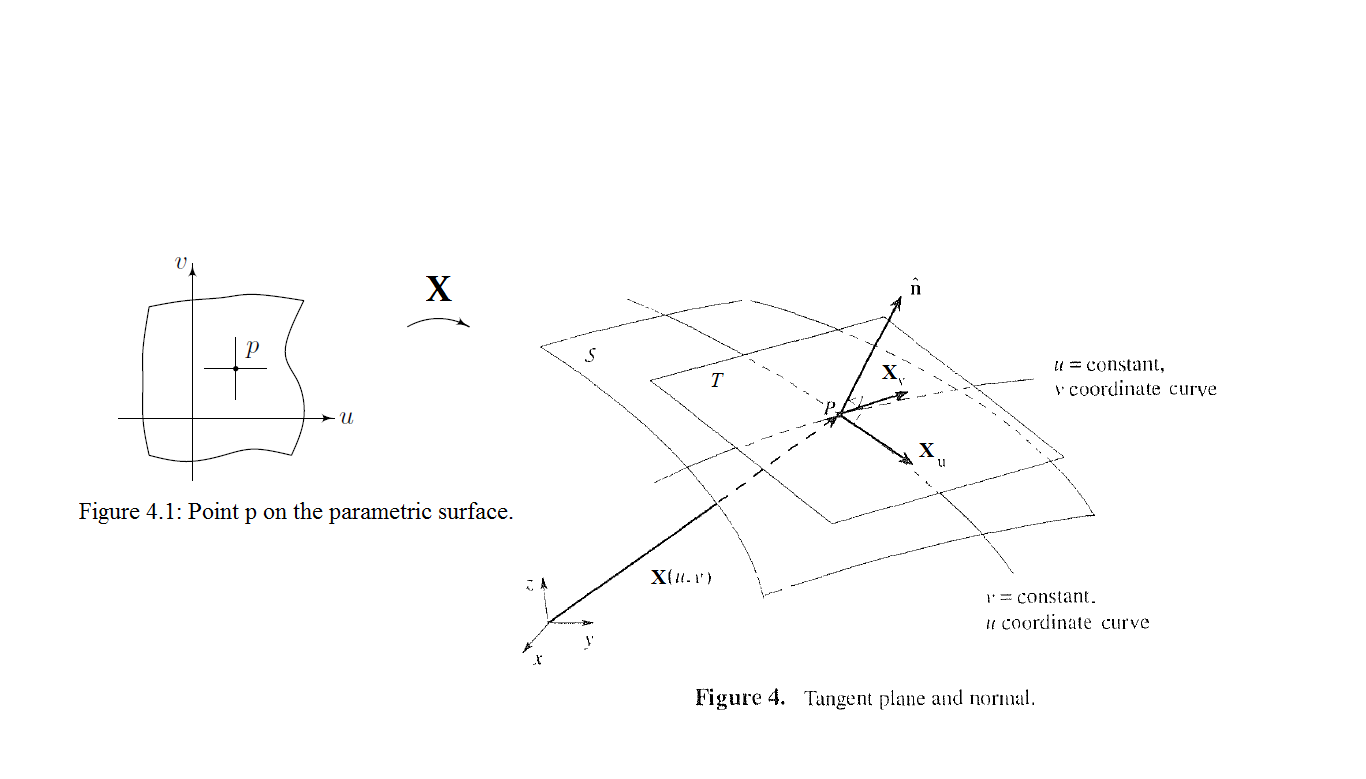
\includegraphics[width=6.0in]{tangentplane.png}
\end{figure}

\begin{equation}
{\bf n} = \frac{ {\bf t_{r}} \times {\bf t_{\theta }}}{||{\bf t_{r}} \times {\bf t_{\theta }}||}
\end{equation}
\begin{equation}
{\bf t_{r}} \times {\bf t_{\theta }} = \bigg[-\frac{\partial h}{\partial z} , -\frac{1}{r}\frac{\partial h}{\partial \theta} ,1\bigg]
\end{equation}
\begin{equation}
||{\bf t_{r}} \times {\bf t_{\theta }}|| = \sqrt{\bigg(\frac{\partial h}{\partial z}\bigg)^2 + \bigg(\frac{1}{r}\frac{\partial h}{\partial \theta}\bigg)^2 + 1}
\end{equation}
\begin{equation}
{\bf n} = \bigg[-\frac{\partial h}{\partial z} , -\frac{1}{r}\frac{\partial h}{\partial \theta} ,1\bigg]\frac{1}{\sqrt{\bigg(\frac{\partial h}{\partial z}\bigg)^2 + \bigg(\frac{1}{r}\frac{\partial h}{\partial \theta}\bigg)^2 + 1}}
\end{equation}
\subsection{Evaluating normal stress and shear stress at the interface.}
rewriting eq(\ref{normalbal}) ,
\begin{equation*}
{\bf n \cdot \tau_{2} \cdot n} - {\bf n\cdot \tau_{1} \cdot n} = \sigma {\bf (\nabla \cdot n)}
\end{equation*}
evaluating ,
\begin{equation}
{\bf {n \cdot \tau \cdot n}} = \sum_{l=1}^{3} (n_{l}{\bf e_{l}}) \cdot \bigg(\sum_{i=1}^{3}\sum_{j=1}^{3} (\tau_{ij}{\bf e_{i}e_{j}})\bigg)\cdot \bigg(\sum_{l=1}^{3} (n_{l}{\bf e_{l}})\bigg)
\end{equation}
\begin{equation*}
{\bf {n \cdot \tau \cdot n}} = \sum_{l=1}^{3} (n_{l}{\bf e_{l}}) \cdot \bigg(\sum_{i=1}^{3}\sum_{j=1}^{3}\sum_{l=1}^{3} (\tau_{ij}  n_{l}({\bf e_{i}e_{j}})\cdot {\bf e_{l}})\bigg)
\end{equation*}
\begin{equation*}
{\bf {n \cdot \tau \cdot n}} = \sum_{l=1}^{3} (n_{l}{\bf e_{l}}) \cdot \bigg(\sum_{i=1}^{3}\sum_{j=1}^{3}\sum_{l=1}^{3} (\tau_{ij}  n_{l}({\bf e_{i}\delta_{jl}})\bigg)
\end{equation*}
\begin{equation*}
{\bf {n \cdot \tau \cdot n}} = \sum_{l=1}^{3} (n_{l}{\bf e_{l}}) \cdot \bigg(\sum_{i=1}^{3}\sum_{j=1}^{3} \tau_{ij}  n_{j}{\bf e_{i}}\bigg)
\end{equation*}
\begin{equation*}
{\bf {n \cdot \tau \cdot n}} = \sum_{l=1}^{3}\sum_{i=1}^{3}\sum_{j=1}^{3} \tau_{ij}n_{j}n_{l}({\bf e_{i} \cdot e_{l}})
\end{equation*}
\begin{equation*}
{\bf {n \cdot \tau \cdot n}} = \sum_{l=1}^{3}\sum_{j=1}^{3} \tau_{lj}n_{j}n_{l} = \sum_{l=1}^{3}n_{l}\sum_{j=1}^{3} \tau_{lj}n_{j}
\end{equation*}
\begin{equation}
{\bf {n \cdot \tau \cdot n}} = n_{1}(\tau_{11}n_{1} + \tau_{12}n_{2} + \tau_{13}n_{3}) +  n_{2}(\tau_{21}n_{1} + \tau_{22}n_{2} + \tau_{23}n_{3}) +  n_{3}(\tau_{31}n_{1} + \tau_{32}n_{2} + \tau_{33}n_{3}) 
\end{equation}

\begin{equation}

n_{1}(\tau_{11}n_{1} + \tau_{12}n_{2} + \tau_{13}n_{3}) = \frac{1}{\bigg(\bigg(\frac{\partial h}{\partial z}\bigg)^2 + \bigg(\frac{1}{r}\frac{\partial h}{\partial \theta}\bigg)^2 + 1\bigg)} 
\bigg[(-p + 2\mu \frac{\partial u_{r}}{\partial r}) + 
 \mu \bigg(\frac{1}{r}\frac{\partial u_{r}}{\partial \theta} -\frac{u_{\theta }}{r}+\frac{\partial u_{\theta }}{\partial r}\bigg)(\frac{-1}{r}\frac{\partial h}{\partial \theta}) + \mu \bigg(\frac{\partial u_{z}}{\partial r} + \frac{\partial u_{r}}{\partial z}\bigg)(\frac{-\partial h}{\partial z})\bigg]
\end{equation}

\begin{equation}
n_{2}(\tau_{21}n_{1} + \tau_{22}n_{2} + \tau_{23}n_{3}) = \frac{\frac{-1}{r}\frac{\partial h}{\partial \theta}}{\bigg(\bigg(\frac{\partial h}{\partial z}\bigg)^2 + \bigg(\frac{1}{r}\frac{\partial h}{\partial \theta}\bigg)^2 + 1\bigg)}
\bigg[\mu \bigg(\frac{1}{r}\frac{\partial u_{r}}{\partial \theta} - \frac{u_{\theta}}{r}+\frac{\partial u_{\theta}}{\partial r}\bigg) +\bigg(-p + 2\mu \bigg(\frac{u_{r}}{r}+\frac{1}{r}\frac{\partial u_{\theta}}{\partial \theta}\bigg)(\frac{-1}{r}\frac{\partial h}{\partial \theta})\bigg)+ \mu \bigg(\frac{1}{r}\frac{\partial u_{z}}{\partial \theta} + \frac{\partial u_{\theta}}{\partial z}\bigg)(\frac{-\partial h}{\partial z})\bigg]
\end{equation}


\begin{equation}
n_{3}(\tau_{31}n_{1} + \tau_{32}n_{2} + \tau_{33}n_{3}) = \frac{\frac{-\partial h}{\partial z}}{\bigg(\bigg(\frac{\partial h}{\partial z}\bigg)^2 + \bigg(\frac{1}{r}\frac{\partial h}{\partial \theta}\bigg)^2 + 1\bigg)}
\bigg[\mu \bigg(\frac{\partial u_{z}}{\partial r} + \frac{\partial u_{r}}{\partial z}\bigg) +\mu \bigg(\frac{1}{r}\frac{\partial u_{z}}{\partial \theta} + \frac{\partial u_{\theta}}{\partial z}\bigg)(\frac{-1}{r}\frac{\partial h}{\partial \theta})+ (-p + 2\mu \frac{\partial u_{z}}{\partial z})(\frac{-\partial h}{\partial z})\bigg]
\end{equation}

\subsection{Evaluation of tangential stress.}
We saw from the stress balance equations that the tangential stress balance across the interface gives,
\begin{equation}
{\bf n \cdot \tau_{2} \cdot t} - {\bf n\cdot \tau_{1} \cdot t} = 0
\end{equation}
where $ {\bf t}$ is a unit tangent vector to the interface surface. This has got 2 components $ {\bf t_{r}}$ and ${\bf t_{\theta}$
\therefore ,
\begin{equation}
{\bf n \cdot \tau_{2} \cdot t_{r}} - {\bf n\cdot \tau_{1} \cdot t_{r}} = 0
\end{equation}
and ,
\begin{equation}
{\bf n \cdot \tau_{2} \cdot t_{\theta }} - {\bf n\cdot \tau_{1} \cdot t_{\theta }} = 0
\end{equation}
evaulating ,
\begin{equation}
{\bf n \cdot \tau \cdot t_{r}} = \sum_{l=1}^{3} (n_{l}{\bf e_{l}}) \cdot \bigg(\sum_{i=1}^{3}\sum_{j=1}^{3} (\tau_{ij}{\bf e_{i}e_{j}})\bigg)\cdot \bigg(\sum_{k=1}^{3} (t_{k}{\bf e_{k}})\bigg)  
\end{equation}
\begin{equation*}
{\bf {n \cdot \tau \cdot t_{r}}} = \sum_{l=1}^{3} (n_{l}{\bf e_{l}}) \cdot \bigg(\sum_{i=1}^{3}\sum_{j=1}^{3}\sum_{k=1}^{3} (\tau_{ij}  t_{k}({\bf e_{i}\delta_{jk}})\bigg)
\end{equation*}
\begin{equation*}
{\bf {n \cdot \tau \cdot t_{r}}} = \sum_{l=1}^{3} (n_{l}{\bf e_{l}}) \cdot \bigg(\sum_{i=1}^{3}\sum_{j=1}^{3} \tau_{ij}  t_{j}{\bf e_{i}}\bigg)
\end{equation*}
\begin{equation*}
{\bf {n \cdot \tau \cdot t_{r}}} = \sum_{l=1}^{3}\sum_{i=1}^{3}\sum_{j=1}^{3} \tau_{ij}t_{j}n_{l}({\bf e_{i} \cdot e_{l}})
\end{equation*}
\begin{equation*}
{\bf {n \cdot \tau \cdot t_{r}}} = \sum_{l=1}^{3}\sum_{j=1}^{3} \tau_{lj}t_{j}n_{l} = \sum_{l=1}^{3}n_{l}\sum_{j=1}^{3} \tau_{lj}t_{j}
\end{equation*}
\begin{equation}
{\bf {n \cdot \tau \cdot t_{r}}} = n_{1}(\tau_{11}t_{1} + \tau_{12}t_{2} + \tau_{13}t_{3}) +  n_{2}(\tau_{21}t_{1} + \tau_{22}t_{2} + \tau_{23}t_{3}) +  n_{3}(\tau_{31}t_{1} + \tau_{32}t_{2} + \tau_{33}t_{3}) 
\end{equation}

\begin{equation*}
{\bf t_{r}} = [t_{r} ,t_{\theta}, t_{z}] = [t_{1} ,t_{2}, t_{3}] =  [{\frac{\partial h}{\partial z}}, 0 , 1]\bigg(\frac{1}{\sqrt{1 + (\frac{\partial {\bf h}}{\partial z}})^2}\bigg)
\end{equation*}

\begin{equation}
n_{1}(\tau_{11}t_{1} + \tau_{12}t_{2} + \tau_{13}t_{3}) = \frac{1}{\bigg(\sqrt{\bigg(\frac{\partial h}{\partial z}\bigg)^2 +  1}\bigg)}\frac{1}{\sqrt{\bigg(\frac{\partial h}{\partial z}\bigg)^2 + \bigg(\frac{1}{r}\frac{\partial h}{\partial \theta}\bigg)^2 + 1}}\bigg[(-p + 2\mu \frac{\partial u_{r}}{\partial r})(\frac{\partial h}{\partial z}) + \mu \bigg(\frac{\partial u_{z}}{\partial r} + \frac{\partial u_{r}}{\partial z}\bigg)\bigg]
\end{equation}

\begin{equation}
 n_{2}(\tau_{21}t_{1} + \tau_{22}t_{2} + \tau_{23}t_{3}) = \frac{1}{\bigg(\sqrt{\bigg(\frac{\partial h}{\partial z}\bigg)^2 +  1}\bigg)}\frac{\frac{-1}{r}\frac{\partial h}{\partial \theta}}{\sqrt{\bigg(\frac{\partial h}{\partial z}\bigg)^2 + \bigg(\frac{1}{r}\frac{\partial h}{\partial \theta}\bigg)^2 + 1}}\bigg[\mu \bigg(\frac{1}{r}\frac{\partial u_{r}}{\partial \theta} -\frac{u_{\theta}}{r}+\frac{\partial u_{\theta}}{\partial r}\bigg)(\frac{\partial h}{\partial z}) + \mu \bigg(\frac{1}{r}\frac{\partial u_{z}}{\partial \theta} + \frac{\partial u_{\theta}}{\partial z}\bigg)\bigg]
\end{equation}


\begin{equation}
n_{3}(\tau_{31}t_{1} + \tau_{32}t_{2} + \tau_{33}t_{3}) = \frac{1}{\bigg(\sqrt{\bigg(\frac{\partial h}{\partial z}\bigg)^2 +  1}\bigg)}\frac{\frac{-\partial h}{\partial z}}{\sqrt{\bigg(\frac{\partial h}{\partial z}\bigg)^2 + \bigg(\frac{1}{r}\frac{\partial h}{\partial \theta}\bigg)^2 + 1}}\bigg[\mu \bigg(\frac{\partial u_{z}}{\partial r} + \frac{\partial u_{r}}{\partial z}\bigg)(\frac{\partial h}{\partial z}) + \bigg(-p + 2\mu \frac{\partial u_{z}}{\partial z}\bigg)\bigg]
\end{equation}
\newline

evaluating ,
\begin{equation}
{\bf n \cdot \tau \cdot t_{\theta}} = \sum_{l=1}^{3} (n_{l}{\bf e_{l}}) \cdot \bigg(\sum_{i=1}^{3}\sum_{j=1}^{3} (\tau_{ij}{\bf e_{i}e_{j}})\bigg)\cdot \bigg(\sum_{k=1}^{3} (t_{k}{\bf e_{k}})\bigg)  
\end{equation}
\begin{equation*}
{\bf {n \cdot \tau \cdot t_{\theta}}} = \sum_{l=1}^{3} (n_{l}{\bf e_{l}}) \cdot \bigg(\sum_{i=1}^{3}\sum_{j=1}^{3}\sum_{k=1}^{3} (\tau_{ij}  t_{k}({\bf e_{i}\delta_{jk}})\bigg)
\end{equation*}
\begin{equation*}
{\bf {n \cdot \tau \cdot t_{\theta}}} = \sum_{l=1}^{3} (n_{l}{\bf e_{l}}) \cdot \bigg(\sum_{i=1}^{3}\sum_{j=1}^{3} \tau_{ij}  t_{j}{\bf e_{i}}\bigg)
\end{equation*}
\begin{equation*}
{\bf {n \cdot \tau \cdot t_{\theta}}} = \sum_{l=1}^{3}\sum_{i=1}^{3}\sum_{j=1}^{3} \tau_{ij}t_{j}n_{l}({\bf e_{i} \cdot e_{l}})
\end{equation*}
\begin{equation*}
{\bf {n \cdot \tau \cdot t_{\theta}}} = \sum_{l=1}^{3}\sum_{j=1}^{3} \tau_{lj}t_{j}n_{l} = \sum_{l=1}^{3}n_{l}\sum_{j=1}^{3} \tau_{lj}t_{j}
\end{equation*}
\begin{equation}
{\bf {n \cdot \tau \cdot t_{\theta}}} = n_{1}(\tau_{11}t_{1} + \tau_{12}t_{2} + \tau_{13}t_{3}) +  n_{2}(\tau_{21}t_{1} + \tau_{22}t_{2} + \tau_{23}t_{3}) +  n_{3}(\tau_{31}t_{1} + \tau_{32}t_{2} + \tau_{33}t_{3}) 
\end{equation}
\begin{equation*}
{\bf t_{\theta }} = [{0 , 1 , \frac{1}{r}\frac{\partial h}{\partial \theta }}]\bigg(\frac{1}{\sqrt{1 + (\frac{1}{r}\frac{\partial {\bf h}}{\partial \theta }})^2}\bigg)
\end{equation*}
\begin{equation*}
[t_{1} ,t_{2}, t_{3}] = [{\frac{1}{r}\frac{\partial h}{\partial \theta }},1,0]\bigg(\frac{1}{\sqrt{1 + (\frac{1}{r}\frac{\partial {\bf h}}{\partial \theta }})^2}\bigg)
\end{equation*}
\begin{equation}
 n_{1}(\tau_{11}t_{1} + \tau_{12}t_{2} + \tau_{13}t_{3}) = \frac{1}{\bigg(\sqrt{\bigg(\frac{1}{r}\frac{\partial h}{\partial \theta}\bigg)^2 +  1}\bigg)}\frac{1}{\sqrt{\bigg(\frac{\partial h}{\partial z}\bigg)^2 + \bigg(\frac{1}{r}\frac{\partial h}{\partial \theta}\bigg)^2 + 1}}\bigg[\bigg(-p + 2\mu \frac{\partial u_{r}}{\partial r}\bigg)(\frac{1}{r}\frac{\partial h}{\partial \theta}) + \mu \bigg(\frac{1}{r}\frac{\partial u_{r}}{\partial \theta} -\frac{u_{\theta}}{r}+\frac{\partial u_{\theta}}{\partial r}\bigg)\bigg]
\end{equation}
\begin{equation}
 n_{2}(\tau_{21}t_{1} + \tau_{22}t_{2} + \tau_{23}t_{3}) = \frac{1}{\bigg(\sqrt{\bigg(\frac{1}{r}\frac{\partial h}{\partial \theta}\bigg)^2 +  1}\bigg)}\frac{\frac{-1}{r}\frac{\partial h}{\partial \theta}}{\sqrt{\bigg(\frac{\partial h}{\partial z}\bigg)^2 + \bigg(\frac{1}{r}\frac{\partial h}{\partial \theta}\bigg)^2 + 1}}\bigg[\mu \bigg(\frac{1}{r}\frac{\partial u_{r}}{\partial \theta} -\frac{u_{\theta}}{r}+\frac{\partial u_{\theta}}{\partial r}\bigg)(\frac{1}{r}\frac{\partial h}{\partial \theta}) + \bigg(-p + 2\mu \bigg(\frac{u_{r}}{r}+\frac{1}{r}\frac{\partial u_{\theta}}{\partial \theta}\bigg)\bigg)\bigg]
\end{equation}
\begin{equation}
n_{3}(\tau_{31}t_{1} + \tau_{32}t_{2} + \tau_{33}t_{3}) = \frac{1}{\bigg(\sqrt{\bigg(\frac{1}{r}\frac{\partial h}{\partial \theta}\bigg)^2 +  1}\bigg)}\frac{\frac{-\partial h}{\partial z}}{\sqrt{\bigg(\frac{\partial h}{\partial z}\bigg)^2 + \bigg(\frac{1}{r}\frac{\partial h}{\partial \theta}\bigg)^2 + 1}}\bigg[\mu \bigg(\frac{\partial u_{z}}{\partial r} + \frac{\partial u_{r}}{\partial z}\bigg)(\frac{1}{r}\frac{\partial h}{\partial \theta})+\mu \bigg(\frac{1}{r}\frac{\partial u_{z}}{\partial \theta} + \frac{\partial u_{\theta}}{\partial z}\bigg)\bigg]
\end{equation}

\end{document}

